\chapter{Zybo}

\section{Zynq}
\subsection{Übersicht}
Der Zynq-7000 ist ein SoC\footnote{System on Chip} der einen 667 MHz Dual-Core ARM Cortex-A9 Prozessor und einem programmierbare Logik enthält, die einem Artix-7 FPGA entspricht.
Der Prozessor und dessen Peripherie befindet sich im \textit{Processing System} oder kurz PS.
Der FPGA-Teil des Zynq wird oft PL oder \textit{Programmable Logic} genannt.
Über den AMBA-Bus kann der Prozessor und auch die PL auf die Peripherie, wie z.B. SPI, GPIO, Ethernet oder auch DDR3 zugreifen.
Das Block Diagramm in der Abbildung \ref{fig:BlockDiagrammZynq} gibt einen guten Überblick über den ganzen SoC.

\begin{figure}[htbp]
	\centering
		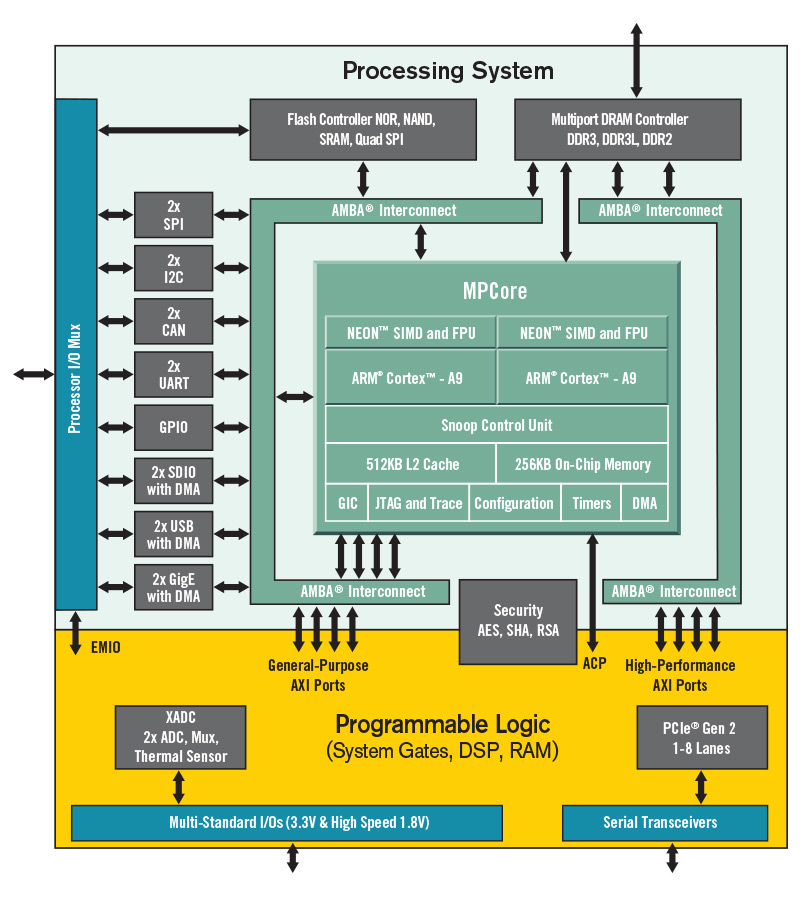
\includegraphics[width=10cm,height=\textheight,keepaspectratio]{images/zynqBlockDiagram.png}
	\caption[Block Diagramm Zynq\-7000]{Block Diagramm Zynq\-7000\footnotemark}
	\label{fig:BlockDiagrammZynq}
\end{figure}
\footnotetext{https://www.xilinx.com/products/silicon-devices/soc/zynq-7000.html}


\subsection{MIO und EMIO}
MIOs sind \textit{Multiplexed Input Output Pins} welche direkt vom Prozessor angesprochen werden können, ohne dass die PL programmiert werden muss.
Die EMIOs sind \textit{\textbf{Extended} Multiplexed Input Output Pins} welche direkt an die PL angeschlossen sind.
Aus diesem Grund können die EMIOs nur verwendet werden, wen die PL entsprechend programmiert wurde.
Diese Arbeit beschränkt sich nur auf die MIOs und das PS.
Im TRM\footnote{Technical Reference Manual} des Zynq\ref{bib:ZynqTechnicalReferenceManual} im Kapitel \textit{''2.5.4 MIO-at-a-Glance Table''} ist eine sehr gute Übersicht über alle möglichen Funktionen der MIOs gegeben.



\section{Standard Zybo Workflow}
Im \textit{Getting Started with Zynq\footnote{https://reference.digilentinc.com/learn/programmable-logic/tutorials/zybo-getting-started-with-zynq/start?redirect=1}} Tutorial von Digilent ist beschrieben, wie man ein einfaches Design für die PL und ein einfaches Programm für das PS erstellt.
Das Tutorial deckt den ganzen Workflow ab.
Dabei werden, z.B. für LED1 bis LED3, auch die EMIOs verwendet.
In Schritt 1 bis 7 wird mit Vivado das Design für die PL erstellt und exportiert.

\textit{Hinweis1:} Die Zybo Toolchain benötigt den standard USB Treiber. Im Kapitel \ref{kapitel:usbTreiber} ist beschrieben, wie der standard USB Treiber wieder installiert werden kann.

\textit{Hinweis2:} Vivado und die Xilinx SDK müssen für dieses Tutorial installiert sein.

Ab Schritt 8 wird beschrieben, wie im XSDK (\textit{Xilinx Standard Development Kit}) ein einfaches ''Hello World'' Programm in C für den Prozessor geschrieben werden kann.
% Das XSDK ist Eclipse mit einem Xylinx Plug-In.

Das XDSK verwendet im Hintergrund das XSCT\footnote{https://www.xilinx.com/html\_docs/xilinx2018\_1/SDK\_Doc/xsct/intro/xsct\_introduction.html} (\textit{Xilinx Software Command-Line Tool}).
Das XDSK kann interaktiv, oder mit Scripts verwendet werden.
% Die Scriptsprache basiert, wie auch Jim-TCL, auf der Sprache TCL.
Wie auch Jim-TCL basiert die verwendete Scriptsprache auf der Sprache TCL.
Wird das ''Hello World'' Programm im XSDK gestartet, erhält man im \textit{SDK Log} Fenster ein detailliertes Log des ausgeführten Script.
In diesem Log kann man nachvollziehen, was beim Download und Start des Programmes alles ausgeführt wird.
